% 4.2 O2 Materials, water and waste. OWNER: Aryan. Sources: deck slides 21-28 (presentation/analysis/*.py),
% D1 atlas (report/analysis/fig_d1_atlas.py). Numbers: claims.csv rows O2a-O2e, Case1, Case2, Method5; claims_report.csv.
\subsection{O2: Water, materials and waste}\label{sec:o2}

% The atlas is a full-width float: declared here so it lands at the top of the next page.
\begin{figure*}[t]\centering
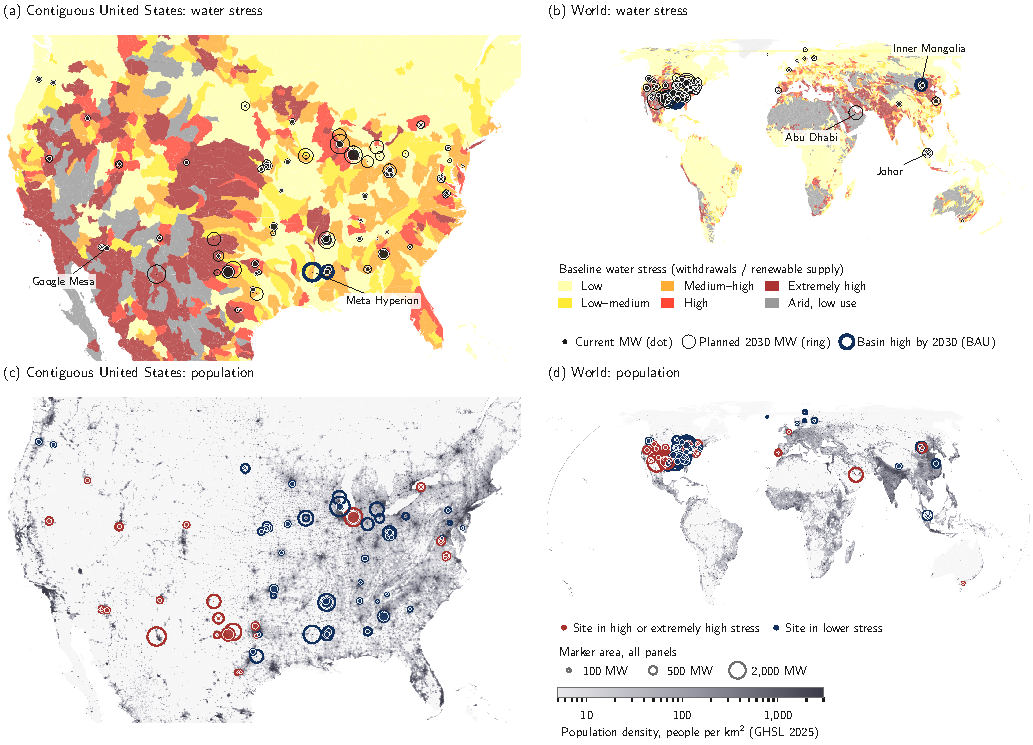
\includegraphics[width=\textwidth]{figs/d1_atlas.pdf}
\caption{Atlas of AI data-centre capacity over water stress and population (deliverable D1). Markers: 96 Epoch AI
sites; filled dot = facility power today, open ring = planned by the end of 2030, area proportional to MW. (a, b) WRI
Aqueduct 4.0 baseline water stress; a thick navy ring marks the four sites whose basin is below ``high'' today but high
or extremely high under the 2030 business-as-usual projection (Meta Hyperion, Amazon Ridgeland and two sites in Inner
Mongolia). (c, d) GHSL 2025 population density; markers are red where the site's basin is in high or extremely high
baseline stress. Grey basins in (a, b) are arid with little water use. Not shown: the Visakhapatnam hub (Section
\ref{sec:cases}), which is not yet in the Epoch data.}
\label{fig:atlas}
\end{figure*}

\paragraph{Where the capacity sits} The 96 sites in the Epoch data add up to 15.1\,GW of facility power today and
50.3\,GW planned by the end of 2030 (\Fig{fig:atlas}). Two things stand out. The rings are much larger than the dots:
most of this capacity is not built yet, so siting decisions are still open. And many of the largest rings sit in red
basins: Stargate in New Mexico, Shackelford and the Texas Panhandle, Stargate UAE in Abu Dhabi, and the Inner Mongolia
cluster. Texas alone plans 7.3\,GW in stressed basins and New Mexico 2.7\,GW. Not every large site is stressed: the
largest planned site, Microsoft's Fairwater campus in Wisconsin (2.7\,GW), sits in a medium--high basin. The population
panels show who lives around these sites: 21 million people within 25\,km of a stressed site (planned sites included),
48 million within 50\,km, out of 106 million within 50\,km of any tracked site.

\begin{figure}[t]\centering
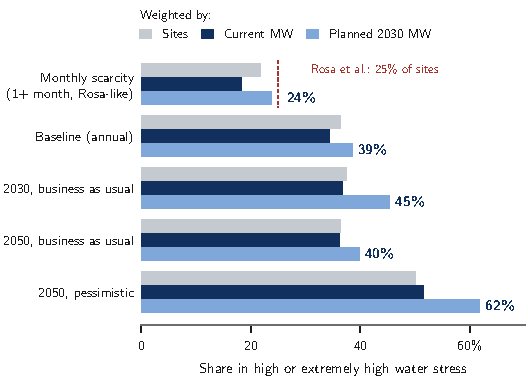
\includegraphics[width=\linewidth]{figs/o2_count_vs_size.pdf}
\caption{Counting sites versus weighting them by size. Share of sites, of current MW and of planned 2030 MW in basins
of high or extremely high water stress, under the baseline and Aqueduct's projections. The red line is Rosa et al.'s
25\%, a share of sites in water-scarce areas.}
\label{fig:count}
\end{figure}

\paragraph{By size, a third of AI capacity is in stressed basins} Counting sites treats a 10\,MW site and a 2\,GW
campus alike, so we weight by power (\Fig{fig:count}). Today 36.5\% of sites and 34.4\% of current MW are in high or
extremely high stress. The planned build-out tilts toward those basins: capacity there grows 3.7-fold to 2030, against
3.1-fold elsewhere, so 38.6\% of the planned MW sits in stressed basins at today's stress levels. Under Aqueduct's 2030
business-as-usual projection the share is 45.4\%. Most of that step comes from two Gulf Coast sites, Meta Hyperion and
Amazon Ridgeland, whose basins sit just under the 40\% line today and cross it in 2030 (+6.4 points); two sites in Inner
Mongolia move from ``arid, low use'' to extremely high (+2.4), and three Utah and Nevada sites drop out ($-1.9$). The
same two Gulf Coast basins fall back by 2050, which is why the 2050 business-as-usual share (39.8\%) is lower than the
2030 one; the 2050 pessimistic case reaches 61.8\%. As a check against Rosa et al.'s monthly method, 21.9\% of our sites
have at least one month in which withdrawals exceed supply, close to their 25\% (2,315 of 9,347 data centres)
\citep{rosa2026}.

\begin{finding}{Finding 2. Weighted by size, 34\% of AI capacity is in stressed basins, 39--45\% of the 2030 plan}
The build-out is heading into dry basins: stressed capacity grows 3.7-fold against 3.1-fold elsewhere. About 21 million
people live within 25\,km of these sites.
\end{finding}

\begin{figure}[t]\centering
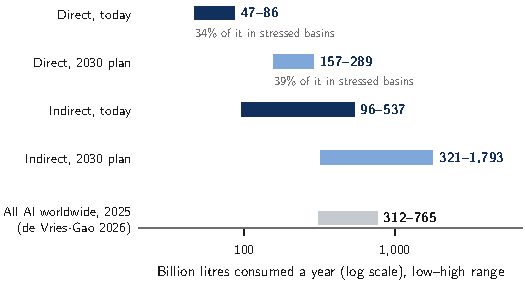
\includegraphics[width=\linewidth]{figs/o2_water_use.pdf}
\caption{Estimated water consumption of the tracked sites, low--high range, today and for the planned 2030 capacity.
Direct: on-site cooling. Indirect: evaporated at the power plants that supply the electricity. Grey: de Vries-Gao's
(2026) estimate for all AI systems worldwide in 2025. Log scale.}
\label{fig:water}
\end{figure}

\paragraph{Most of the water is used at power plants} Today's 15\,GW consume an estimated 143--624 billion litres a
year, and the 2030 plan 478--2,082 billion (\Fig{fig:water}). Between 67 and 86\% of it is \emph{indirect}: water
evaporated at the power plants, not at the data centre. On-site cooling water in stressed basins comes to 16--30
billion litres a year today and 61--111 billion by 2030. Our range for today overlaps de Vries-Gao's independent
estimate of 312--765 billion litres for all AI systems worldwide in 2025 \citep{devriesgao2026}. The width of the range
comes mostly from the grid factor (1.04 against 4.52\,L/kWh). Sites matter more than totals here: the Epoch sites that
report water imply anything from 0.001 to 7\,L per facility kWh (at an assumed 80\% load), against our range of
0.51--0.73\,L for on-site use. Cooling design, not size, decides a site's direct water.

\begin{figure}[t]\centering
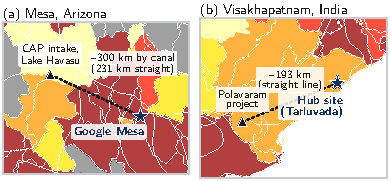
\includegraphics[width=\linewidth]{figs/o2_case_locator.pdf}
\caption{The two case studies and their water sources, over Aqueduct baseline water stress (same colours as
\Fig{fig:atlas}). Star: data centre; triangle: water source. Mesa's Colorado River water reaches the Phoenix area
through the Central Arizona Project canal; Visakhapatnam's promised source is the Polavaram project.}
\label{fig:cases}
\end{figure}

\paragraph{Case 1: Google Mesa, a desert site whose water travels 300\,km}\label{sec:cases} Google's Mesa campus
(183\,MW today, 237\,MW planned) sits in a basin of extremely high stress, where withdrawals exceed renewable supply in
all twelve months of the year. Google's agreement with the city, reported in 2020, guarantees 1 million US gallons a day
and allows up to 4 million, about 15 million litres a day or 5.5 billion litres a year \citep{sattiraju2020,solon2021}.
By our method, on-site use for 237\,MW would be 0.7--1.4 billion litres a year, close to the guaranteed volume (1.4
billion); the ceiling is four to seven times our estimate, so it is a permission, not a measure of use. Actual use is
not disclosed. More than half of Mesa's water (53\%) is Colorado River water delivered through the Central Arizona
Project canal, about 300\,km long (231\,km in a straight line from the intake at Lake Havasu); 40\% comes from the Salt
and Verde rivers and 7\% from groundwater \citep{mesa2026,reclamation_cap}. That river is being cut: in August 2026 the
federal government reduced Lower Basin allocations by 1.25 million acre-feet a year for 2027--2028
\citep{mesa2026,reclamation2026}. Local politics has noticed. When the city approved its next, Facebook-linked data centre in
2021, Vice Mayor Jenn Duff cast the only vote against, calling data centres ``an irresponsible use of our water''
\citep{solon2021}. Her vote concerned that project, not Google's.

\paragraph{Case 2: Visakhapatnam, a gigawatt hub in a city already short of water} Google, with AdaniConneX and
Airtel, plans a 1\,GW AI hub near Visakhapatnam, worth about US\$15 billion \citep{google2025,federal2026}, on three campuses
(Tarluvada, Adavivaram and Rambilli); the foundation stone was laid at Tarluvada on 28 April 2026 \citep{deccan2025,mongabay2026}. The city already receives about 410 of the 480 million litres a day it needs, a
shortfall of 15\% \citep{federal2026}. The environmental clearance does not disclose the site's water use in operation
\citep{mongabay2026}. The state government says water will come by dedicated pipeline from the Polavaram project, about
190\,km away in a straight line, and the companies say the site will be air-cooled; residents have protested under the
slogan ``We cannot drink data'' \citep{federal2026}. Our check places the Tarluvada site in a medium--high stress basin (20--40\%), with no month
in which withdrawals exceed supply. Air cooling removes most of the on-site water, but not the water at the power
plants: for 1\,GW our range is 17--98 million litres a day, equal to 4--24\% of the city's present supply. This compares
scale only. Those plants need not draw on the city's supply, and the grid factors are US-derived. Why this city was chosen,
and whether water stress counted, is the subject of Section~\ref{sec:siting}.

\begin{figure}[t]\centering
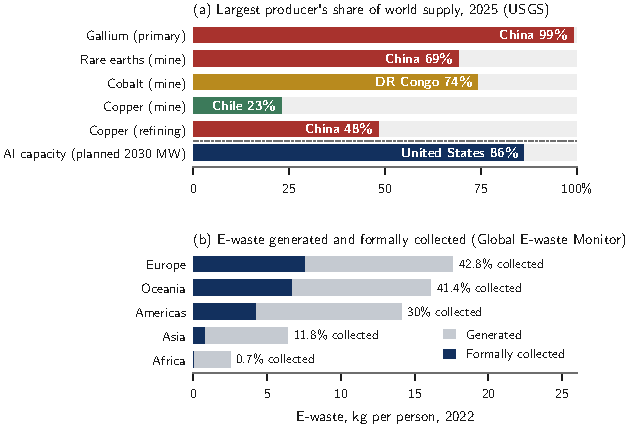
\includegraphics[width=\linewidth]{figs/o2_materials_ewaste.pdf}
\caption{Minerals are mined in a few countries; e-waste collection is very uneven. (a) Share of world supply from
the largest producer, 2025, with the US share of planned AI capacity for comparison. (b) E-waste generated per person
in 2022 and the share formally collected.}
\label{fig:materials}
\end{figure}

\paragraph{Minerals and e-waste} The hardware depends on minerals whose supply is concentrated
(\Fig{fig:materials}). In 2025 China produced 99\% of the world's primary gallium, 69\% of mined rare earths and 48\%
of refined copper; DR Congo mined 74\% of cobalt and Chile 23\% of copper \citep{usgs2026}. The demand sits elsewhere:
86\% of the planned AI capacity in our data is in the United States. Supply can be cut. China's December 2024 ban on
gallium and germanium exports to the United States was suspended under MOFCOM Announcement 72 until 27 November 2026
\citep{usgs2026,mofcom2025}; as of late November 2026 no official notice has extended the suspension (though press reports suggest a possible extension into early 2027), leaving near-term supply uncertain. At the end of the chain, the world
generated 62 million tonnes of e-waste in 2022, of which 22\% was formally collected \citep{balde2024}. Collection
ranges from 42.8\% in Europe to 0.7\% in Africa. The USGS does not break out the share of these minerals that goes
to AI, and the e-waste data cover all electronics, so this part of the analysis shows concentration, not AI's
share.

\paragraph{Against the global boundary} The Earth3 model treats freshwater as one global number: withdrawals below
3,000\,\kmc\ a year are safe, above 4,000\,\kmc\ high-risk \citep{collste2018}. The 2030 plan's 0.5--2.1\,\kmc\ is
0.02--0.07\% of the safe limit. The comparison mixes our consumption with a withdrawal limit, and withdrawals would be
larger, but even several times more would still be well under 1\%.

\begin{finding}{Finding 3. Against a global boundary AI's water barely registers; in a basin it does}
Under 0.1\% of Earth3's freshwater limit, yet 12 of 12 months over supply in Mesa's basin, and a planned gigawatt hub
in a city already 15\% short. A single global number averages away exactly where the pressure is: AI's water has to be
judged basin by basin.
\end{finding}
